% ============================================================
%  RR-LineBundles-Picard.tex
%  Riemann--Roch on CP^1 via Holomorphic Line Bundles,
%  the Picard Group, and the Winding Form
%  Author: Ji, Yonghyeon
% ============================================================

\documentclass[11pt,openany]{article}

% kotex needs cjk fallback when Korean OTF fonts are absent
%\PassOptionsToPackage{cjk}{kotex}
\usepackage{kotex}
\usepackage{mathtools, commath}
% Packages for formatting
\usepackage[margin=1in]{geometry}
\usepackage{fancyhdr}
\usepackage{enumerate}
\usepackage{graphicx}
\usepackage{kotex}
\usepackage{arydshln} % Include this package
\usepackage{bbding}
\usepackage{amsmath}
\usepackage{amsthm}
\usepackage[dvipsnames,table]{xcolor}
\usepackage{amssymb, amsfonts}
\usepackage{wasysym}
\usepackage{footnote}
\usepackage{tablefootnote}
\usepackage{arydshln} % Include this package
\usepackage{framed}
\usepackage{physics}

% Fonts
\usepackage[T1]{fontenc}
\usepackage[utf8]{inputenc}
\usepackage{newpxtext,newpxmath}
\usepackage{sectsty}

% Define colors
\definecolor{TealBlue1}{HTML}{0077c2}
\definecolor{TealBlue2}{HTML}{00a5e6}
\definecolor{TealBlue3}{HTML}{b3e0ff}
\definecolor{TealBlue4}{HTML}{00293c}
\definecolor{TealBlue5}{HTML}{e6f7ff}

\definecolor{thmcolor}{RGB}{231, 76, 60}
\definecolor{defcolor}{RGB}{52, 152, 219}
\definecolor{lemcolor}{RGB}{155, 89, 182}
\definecolor{corcolor}{RGB}{46, 204, 113}
\definecolor{procolor}{RGB}{241, 196, 15}

\usepackage{color,soul}
\usepackage{soul}
\newcommand{\mathcolorbox}[2]{\colorbox{#1}{$\displaystyle #2$}}
\usepackage{cancel}
\newcommand\crossout[3][black]{\renewcommand\CancelColor{\color{#1}}\cancelto{#2}{#3}}
\newcommand\ncrossout[2][black]{\renewcommand\CancelColor{\color{#1}}\cancel{#2}}

\usepackage{hyperref}
\usepackage{booktabs}

% Chapter formatting
\definecolor{titleTealBlue}{RGB}{0,53,128}
\usepackage{titlesec}
\titleformat{\section}
{\normalfont\sffamily\LARGE\bfseries\color{titleTealBlue!100!gray}}{\thesection}{1em}{}
\titleformat{\subsection}
{\normalfont\sffamily\Large\bfseries\color{titleTealBlue!85!gray}}{\thesubsection}{1em}{}
\titleformat{\subsubsection}
{\normalfont\sffamily\Large\bfseries\color{titleTealBlue!70!gray}}{\thesubsubsection}{1em}{}

%Tcolorbox
\usepackage[most]{tcolorbox}
\usepackage{multirow}
\usepackage{multicol}
\usepackage{blindtext}

\usepackage[linesnumbered,ruled]{algorithm2e}
\usepackage{algpseudocode}
\usepackage{setspace}
\SetKwComment{Comment}{/* }{ */}
\SetKwProg{Fn}{Function}{:}{end}
\SetKw{End}{end}
\SetKw{DownTo}{downto}

% Define a new environment for algorithms without line numbers
\newenvironment{algorithm2}[1][]{
	% Save the current state of the algorithm counter
	\newcounter{tempCounter}
	\setcounter{tempCounter}{\value{algocf}}
	% redefine the algorithm numbering (remove prefix)
	\renewcommand{\thealgocf}{}
	\begin{algorithm}
	}{
	\end{algorithm}
	% Restore the algorithm counter state
	\setcounter{algocf}{\value{tempCounter}}
}

\usepackage{adjustbox}
% Header and footer formatting
\pagestyle{fancy}
\fancyhead{}
\fancyhf{}
\rhead{\textcolor{TealBlue2}{\large\textbf{리만의 복소해석을 토대로 얻는 내 수학적 시야 (2기)}}}%\rule{3cm}{0.4pt}}
\lhead{\textcolor{TealBlue2}{\large\textbf{수학의 즐거움, Enjoying Math}}}
% Define footer
%\newcommand{\footer}[1]{
%\begin{flushright}
%	\vspace{2em}
%	\includegraphics[width=2.5cm]{school_logo.jpg} \\
%	\vspace{1em}
%	\textcolor{TealBlue2}{\small\textbf{#1}}
%\end{flushright}
%}
%\rfoot{\large Department of Information Security, Cryptogrphy and Mathematics, Kookmin Uni.\includegraphics[height=1.5cm]{school_logo.jpg}}
\fancyfoot{}
\fancyfoot[C]{-\thepage-}

% Note: riemann-animate omitted (requires animation PDFs in sibling directory)
\usepackage{tcolorbox}
\tcbset{colback=white, arc=5pt}

\definecolor{axiomcolor}{HTML}{a88bfa}
\definecolor{defcolor}{RGB}{52, 152, 219}
\definecolor{procolor}{RGB}{241, 196, 15}
\definecolor{thmcolor}{RGB}{231, 76, 60}
\definecolor{lemcolor}{RGB}{155, 89, 182}
\definecolor{corcolor}{RGB}{46, 204, 113}
\definecolor{execolor}{RGB}{90, 128, 127}

% Define a new command for the custom tcolorbox
\newcommand{\axiombox}[2][]{%
	\begin{tcolorbox}[colframe=axiomcolor, title={\color{white}\bfseries #1}]
		#2
	\end{tcolorbox}
}

\newcommand{\defbox}[2][]{%
	\begin{tcolorbox}[colframe=defcolor, title={\color{white}\bfseries #1}]
		#2
	\end{tcolorbox}
}

\newcommand{\lembox}[2][]{%
	\begin{tcolorbox}[colframe=lemcolor, title={\color{white}\bfseries #1}]
		#2
	\end{tcolorbox}
}

\newcommand{\probox}[2][]{%
	\begin{tcolorbox}[colframe=procolor, title={\color{white}\bfseries #1}]
		#2
	\end{tcolorbox}
}

\newcommand{\thmbox}[2][]{%
	\begin{tcolorbox}[colframe=thmcolor, title={\color{white}\bfseries #1}]
		#2
	\end{tcolorbox}
}

\newcommand{\corbox}[2][]{%
	\begin{tcolorbox}[colframe=corcolor, title={\color{white}\bfseries #1}]
		#2
	\end{tcolorbox}
}



\usepackage{amsthm}

% Define custom theorem styles
\newtheoremstyle{dotless} % Name of the style
{3pt} % Space above
{3pt} % Space below
{\itshape} % Body font
{} % Indent amount
{\bfseries} % Theorem head font
{} % Punctuation after theorem head
{2.5mm} % Space after theorem head
{} % Theorem head spec

\newtheoremstyle{definitionstyle} % Name of the style
{3pt} % Space above
{3pt} % Space below
{} % Body font
{} % Indent amount
{\bfseries} % Theorem head font
{.} % Punctuation after theorem head
{2.5mm} % Space after theorem head
{} % Theorem head spec

% Applying custom styles
%\theoremstyle{dotless}
\newtheorem{theorem}{Theorem} % Theorem environment with section-wise numbering
\newtheorem*{theorem*}{Theorem} % Theorem environment with section-wise numbering
\newtheorem*{lemma*}{Lemma} % Theorem environment with section-wise numbering
\newtheorem*{proposition*}{Proposition} % Theorem environment with section-wise numbering
\newtheorem*{corollary*}{Corollary} % Theorem environment with section-wise numbering
\newtheorem{proposition}[theorem]{Proposition} % Theorem environment with section-wise numbering
\newtheorem{lemma}[theorem]{Lemma} % Lemma shares the counter with theorem
\newtheorem{corollary}[theorem]{Corollary} % Corollary shares the counter with theorem

\theoremstyle{definitionstyle}
\newtheorem*{observation}{\textcolor{Magenta}{Observation}}
\newtheorem{claim}{Claim}
\newtheorem{definition}{Definition} % Definition shares the counter with theorem
\newtheorem{example}{Example} % Example shares the counter with theorem
\newtheorem{exercise}{{Exercise}} % Example shares the counter with theorem
\newtheorem{remark}{Remark} % Remark shares the counter with theorem
\newtheorem*{note}{Note}

\newtheorem*{axiom*}{Axiom}
\newtheorem*{definition*}{Definition} % Definition shares the counter with theorem
\newtheorem*{example*}{Example} % Example shares the counter with theorem
\newtheorem*{exercise*}{\textcolor{teal}{Exercise}} % Example shares the counter with theorem
\newtheorem*{remark*}{Remark} % Remark shares the counter with theorem


\usepackage{tikz}
\usepackage{tikz-cd}
\usepackage{tikz-3dplot}
\usepackage{pgfplots}
\pgfplotsset{compat=newest} % Adjust to your version of pgfplots
\def\Circlearrowleft{\ensuremath{%
		\rotatebox[origin=c]{180}{$\circlearrowleft$}}}
\def\Circlearrowright{\ensuremath{%
		\rotatebox[origin=c]{180}{$\circlearrowright$}}}
\def\CircleArrowleft{\ensuremath{%
		\reflectbox{\rotatebox[origin=c]{180}{$\circlearrowleft$}}}}
\def\CircleArrowright{\ensuremath{%
		\reflectbox{\rotatebox[origin=c]{180}{$\circlearrowright$}}}}
\usetikzlibrary{
	3d, % For 3D drawing
	angles,
	arrows,
	arrows.meta,
	backgrounds,
	bending,
	calc,
	decorations.pathmorphing,
	decorations.pathreplacing,
	decorations.markings,
	fit,
	matrix,
	patterns,
	patterns.meta,
	positioning,
	quotes,
	shadows,
	shapes,
	shapes.geometric,
	tikzmark
}
\tikzset{
	% single mid‐path arrow
	mid arrow/.style={
		decoration={
			markings,
			mark=at position 0.5 with {\arrow{Stealth[scale=1.2]}}
		},
		postaction={decorate},
	},
	% style for field arrows
	field arrow/.style={
		-{Stealth[scale=1.0]},
		thick,
		blue!70!black,
	},
}
\newcommand{\ie}{\textnormal{i.e.}}
\newcommand{\rsa}{\mathsf{RSA}}
\newcommand{\rsacrt}{\mathsf{RSA}\textendash\mathsf{CRT}}
\newcommand{\inv}[1]{#1^{-1}}

%New Command
%\newcommand{\set}[1]{\left\{#1\right\}}
\newcommand{\N}{\mathbb{N}}
\newcommand{\Z}{\mathbb{Z}}
\newcommand{\Q}{\mathbb{Q}}
\newcommand{\R}{\mathbb{R}}
\newcommand{\cR}{\mathcal{R}}
\newcommand{\C}{\mathbb{C}}
\newcommand{\F}{\mathbb{F}}
\newcommand{\nbhd}{\mathcal{N}}
\newcommand{\Log}{\operatorname{Log}}
\newcommand{\Arg}{\operatorname{Arg}}
%\newcommand{\pv}{\operatorname{P.V.}}

\newcommand{\of}[1]{\left( #1 \right)} 
%\newcommand{\abs}[1]{\left\lvert #1 \right\rvert}
%\newcommand{\norm}[1]{\left\| #1 \right\|}

\newcommand{\sol}{\textcolor{magenta}{\bf Sol}}
\newcommand{\conjugate}[1]{\overline{#1}}

%\newcommand{\res}{\operatorname{res}}
%\DeclareMathOperator*{\Res}{\operatorname{Res}}

%\renewcommand{\Re}{\operatorname{Re}}
%\renewcommand{\Im}{\operatorname{Im}}

\newcommand{\cyclic}[1]{\langle #1 \rangle}
\newcommand{\uniform}{\overset{\$}{\leftarrow}}
\newcommand{\xmark}{\textcolor{red}{\XSolidBrush}}
\newcommand{\vmark}{\textcolor{green!75!black}{\CheckmarkBold}}

\newcommand{\gen}[1]{\langle #1 \rangle}
\newcommand{\Gen}[1]{\left\langle #1 \right\rangle}

\newcommand{\img}[1]{\text{Img}(#1)}
\newcommand{\Img}[1]{\text{Img}\left(#1\right)}
\newcommand{\preimg}[1]{\text{Img}^{-1}(#1)}
\newcommand{\Preimg}[1]{\text{Img}^{-1}\left(#1\right)}

\newcommand{\relation}{\mathrel{\mathcal{R}}}
\newcommand{\injection}{\rightarrowtail}
\newcommand{\surjection}{\twoheadrightarrow}
\newcommand{\id}{\textnormal{id}}

\newcommand{\eqclass}[1]{\left[#1\right]}

% Define custom colors for O and X
\newcommand{\yes}{\textcolor{blue}{\bf \fullmoon}}
\newcommand{\no}{\textcolor{red}{\bf \texttimes}}

\DeclarePairedDelimiter\ceil{\lceil}{\rceil}
\DeclarePairedDelimiter\floor{\lfloor}{\rfloor}
%\renewcommand{\floor}[#1]{\lfloor #1\rfloor}
%\newcommand{\Floor}[#1]{\left\lfloor #1\right\rfloor}
%\newcommand{\ceil}[#1]{\lceil #1\rceil}
%\newcommand{\Ceil}[#1]{\left\lceil #1\right\rceil}

\newcommand{\topology}{\mathscr{T}}
\newcommand{\sequence}[1]{\langle #1\rangle}

% Topology
%\newcommand{\nbhd}{\mathcal{N}}

% Linear Algebra
\newcommand{\Span}{\operatorname{\normalfont span}}
\newcommand{\basis}{\mathcal{B}}
\newcommand{\card}[1]{\text{\normalfont card}(#1)}

\renewcommand{\vec}[1]{\mathbf{#1}}
\renewcommand{\emph}[1]{\textbf{#1}}
\setstretch{1.25}

% ── Custom colors (matching reference) ──────────────────────
\definecolor{titleblue}{RGB}{22,72,130}
\definecolor{softgray}{RGB}{245,247,250}
\definecolor{rulegray}{RGB}{210,215,222}
\definecolor{noteblue}{RGB}{232,241,252}
\definecolor{warnred}{RGB}{252,237,237}
\definecolor{greenbox}{RGB}{236,247,238}

% ── Framed environments ──────────────────────────────────────
\newenvironment{infobox}{%
  \def\FrameCommand{\fboxrule=0.8pt \fboxsep=8pt \colorbox{noteblue}}%
  \MakeFramed{\advance\hsize-\width \FrameRestore}}{\endMakeFramed}

\newenvironment{warningbox}{%
  \def\FrameCommand{\fboxrule=0.8pt \fboxsep=8pt \colorbox{warnred}}%
  \MakeFramed{\advance\hsize-\width \FrameRestore}}{\endMakeFramed}

\newenvironment{greenboxenv}{%
  \def\FrameCommand{\fboxrule=0.8pt \fboxsep=8pt \colorbox{greenbox}}%
  \MakeFramed{\advance\hsize-\width \FrameRestore}}{\endMakeFramed}

% ── Line bundle / divisor macros ────────────────────────────
\newcommand{\CP}{\mathbb{CP}}
\newcommand{\CPone}{\CP^1}
\newcommand{\OO}{\mathcal{O}}
\newcommand{\MM}{\mathcal{M}}
\newcommand{\Div}{\operatorname{Div}}
\newcommand{\Pic}{\operatorname{Pic}}
\newcommand{\Prin}{\operatorname{Prin}}
\newcommand{\degd}{\operatorname{deg}}
\newcommand{\ellD}{\ell}
\newcommand{\ord}{\operatorname{ord}}
\newcommand{\into}{\hookrightarrow}
\newcommand{\surj}{\twoheadrightarrow}
\renewcommand{\div}{\operatorname{div}}
% \set is already defined by commath; use \renewcommand to override
\renewcommand{\set}[1]{\left\{#1\right\}}

% ── Winding form macros ─────────────────────────────────────
% \wform{f}  produces  df/f  (the 1-form, no 1/2πi)
\newcommand{\wform}[1]{\dfrac{d#1}{#1}}
% \wind{\gamma}{f}  produces  (1/2πi)∮_γ d(f)/f
% For compound arguments (e.g. z^n) wrap: \wind{\gamma}{(z^n)}
\newcommand{\wind}[2]{\dfrac{1}{2\pi i}\oint_{#1}\dfrac{d\!\left(#2\right)}{#2}}

% ── Full-function display ────────────────────────────────────
% \fullfunction may already be defined; use \providecommand then redefine
\providecommand{\fullfunction}[5]{}
\renewcommand{\fullfunction}[5]{%
  \begin{array}{r@{\;}c@{\;}l}
    #1\colon #2 &\longrightarrow& #3 \\[2pt]
    #4          &\longmapsto&    #5
  \end{array}
}

% Start section numbering at 0
\setcounter{section}{-1}

% ============================================================
\begin{document}
\pagenumbering{arabic}

% ── Title ───────────────────────────────────────────────────
\begin{center}
  \Huge\textbf{Riemann--Roch Theorem via Holomorphic Line Bundles}\\[6pt]
  \Huge\textbf{and the Picard Group on $\CPone$}\\
  \vspace{0.6em}
  \large Ji, Yonghyeon\\
  \vspace{0.4em}
  \normalsize \today
\end{center}

\noindent
We develop the Riemann--Roch theorem on $\CPone$ through the following topics.
\begin{itemize}
  \item The winding form $\dfrac{df}{f}$ as the universal counting tool
  \item Holomorphic line bundles $\OO(n)$ and their classification
  \item Divisors and the associated line bundle $\OO(D)$
  \item The Picard group $\Pic(\CPone)\cong\mathbb{Z}$ via winding numbers
  \item The canonical bundle $K_{\CPone}=\OO(-2)$ and Serre duality
  \item Riemann--Roch on $\CPone$ as a winding-number balance
\end{itemize}

\medskip

\begin{infobox}
\textbf{Riemann--Roch Theorem.}
On a compact Riemann surface $X$ of genus $g$,
\[
  \ell(D) - \ell(K-D) = \deg D + 1 - g,
\]
where $D$ is a divisor, $K$ is a canonical divisor, and $\ell(D)=\dim_\C L(D)$.
For $X=\CPone$ one has $g=0$, giving
\[
  \ell(D) - \ell(K-D) = \deg D + 1.
\]
\textbf{Guiding idea.}
The integers $\deg D$ and $\deg K$ are \emph{winding numbers} — values of the integral
$\dfrac{1}{2\pi i}\oint\dfrac{df}{f}$.
Every quantity in the formula is assembled from this single primitive.
\end{infobox}

\newpage
\tableofcontents

\subsection*{Notation}
\begin{itemize}
  \item[$\OO(X)$] Global holomorphic functions on $X$.
    \quad\textbf{Warning:} $\OO(X)$ uses a \emph{manifold} argument and denotes a
    function ring; $\OO(n)$ uses an \emph{integer} argument and denotes a line bundle.
    These must never be confused.
  \item[$\OO(n)$] Holomorphic line bundle on $\CPone$ with transition function $z^n$
  \item[$\MM(X)$] Meromorphic functions on $X$; $\MM(X)^\times = \MM(X)\setminus\{0\}$
  \item[$H^0(X,\mathcal{L})$] Space of global holomorphic sections of line bundle $\mathcal{L}$
  \item[$L(D)$] Riemann--Roch space $\{f\in\MM(\CPone)^\times:\div(f)+D\ge0\}\cup\{0\}$
  \item[$\ell(D)$] $\dim_\C L(D)$
  \item[$\Pic(X)$] Picard group: isomorphism classes of holomorphic line bundles
  \item[$c_1(\mathcal{L})$] First Chern class $= \deg\mathcal{L} =$ winding number of transition function
  \item[$\dfrac{df}{f}$]
    \textbf{Winding form} of $f$: globally well-defined logarithmic derivative.
    Locally $\dfrac{df}{f}=d(\log f)$ wherever a branch of $\log f$ exists,
    but that equality is only a local mnemonic, not a global definition.
  \item[$\dfrac{1}{2\pi i}\oint_\gamma\dfrac{df}{f}$]
    Winding number of $f$ along $\gamma$;
    equals $\ord_p(f)$ when $\gamma$ is a small loop encircling only $p$
\end{itemize}

% ============================================================
%  Section 0: The Winding Form
% ============================================================
\newpage
\section{The Winding Form}
\label{sec:winding}

\medskip\noindent
\emph{Every integer appearing in this note — order of a zero or pole, degree of a
divisor, winding number of a transition function — is the value of one integral.
This section introduces that integral.}

% ------ §0.0  Coordinates ---------------------------------
\subsection*{Coordinates on $\CPone$}
\label{subsec:coords}

\defbox[Complex Projective Line]{%
\begin{definition}
$\CPone = (\C^2\setminus\{0\})/{\sim}$
where $(Z_0,Z_1)\sim(\lambda Z_0,\lambda Z_1)$ for all $\lambda\in\C^\times$.
The class is denoted $[Z_0:Z_1]$.
\end{definition}}

\begin{remark}
The two standard affine charts:
\[
  U_0=\{Z_0\neq 0\},\quad z=Z_1/Z_0,
  \qquad
  U_\infty=\{Z_1\neq 0\},\quad w=Z_0/Z_1.
\]
On $U_0$: $[Z_0:Z_1]=[1:z]$.
On $U_\infty$: $[Z_0:Z_1]=[w:1]$.
Overlap $U_0\cap U_\infty\cong\C^\times$: $w=1/z$.
Point at infinity: $\infty=[0:1]\in U_\infty$ at $w=0$.
\end{remark}

% ------ §0.1  Logarithmic derivative ---------------------
\subsection{The Logarithmic Derivative}
\label{subsec:logderiv}

\defbox[Winding Form]{%
\begin{definition}
For $f\in\MM(U)^\times$, the \textbf{winding form} of $f$ is the meromorphic $1$-form
\[
  \wform{f} = \frac{df}{f}.
\]
\end{definition}}

\begin{observation}
On any open set where a holomorphic branch $\log f$ exists,
$\dfrac{df}{f}=d(\log f)$ holds locally.
However, $\dfrac{df}{f}$ is globally well-defined on all of $U$ without branch choice:
the ambiguity in $\log f$ (shifts by $2\pi i\mathbb{Z}$) vanishes upon differentiation.
The expression ``$d(\log f)$'' is therefore only a local mnemonic.
\end{observation}

\medskip

{\color{blue}\textbf{Key computation.}}
For $f=z^n$ ($n\in\mathbb{Z}$):
\[
  \frac{d(z^n)}{z^n} = \frac{nz^{n-1}\,dz}{z^n} = n\,\frac{dz}{z}.
\]
Integrating around a small circle $\gamma$ centred at $0$:
\[
  \wind{\gamma}{(z^n)}
  = \frac{n}{2\pi i}\oint_\gamma\frac{dz}{z} = n.
\]
This integer $n$ is the order of $f$ at $0$
(positive for a zero, negative for a pole)
and simultaneously the winding number of the map $z\mapsto z^n$ around the origin.

% ------ §0.2  Winding number = order --------------------
\subsection{Winding Number = Order}
\label{subsec:windord}

\defbox[Order via Winding]{%
\begin{definition}
For $f\in\MM(X)^\times$ and $p\in X$, the \textbf{order of $f$ at $p$} is
\[
  \ord_p(f) := \wind{\gamma_p}{f}
  = \frac{1}{2\pi i}\oint_{\gamma_p}\frac{df}{f},
\]
where $\gamma_p$ is a small loop encircling $p$ once counterclockwise.
\end{definition}}

\begin{observation}
Write $f=z^m u$ near $p$, with local coordinate $z$ centred at $p$ and $u(p)\neq 0$.
Then
\[
  \frac{df}{f} = m\,\frac{dz}{z}+\frac{du}{u}.
\]
On a sufficiently small \emph{simply connected} disk $\Delta$ around $p$ where $u$
is nonvanishing, $u$ admits a holomorphic logarithm, so $\dfrac{du}{u}=d(\log u)$
is exact on $\Delta$; hence $\oint_{\gamma_p}\dfrac{du}{u}=0$.
Only the pole of $\dfrac{dz}{z}$ contributes, giving $\ord_p(f)=m$.
\end{observation}

% ------ §0.3  Global Stokes argument --------------------
\subsection{The Global Stokes Argument: $\deg\div(f)=0$}
\label{subsec:degzero}

\lembox{%
\begin{lemma}
\label{lem:degzero}
For $f\in\MM(X)^\times$ on a compact Riemann surface $X$,
\[
  \sum_{p\in X}\ord_p(f) = 0.
\]
\end{lemma}}

\begin{proof}
Let $p_1,\ldots,p_N$ be the zeros and poles of $f$.
Choose pairwise disjoint closed disks $D_j(r)$ around each $p_j$
with boundary circles $C_j(r)=\partial D_j(r)$, and set
\[
  X_r := X\setminus\bigcup_{j=1}^N D_j(r).
\]
On $X_r$, the function $f$ is holomorphic and nonvanishing, so locally $f=e^g$ for a
holomorphic branch $g$.  Thus $\omega:=\dfrac{df}{f}=dg$ is locally exact, and
\[
  d\omega = d(dg) = 0
\]
since $d\circ d=0$.  By Stokes:
\[
  0 = \int_{X_r}d\omega = \int_{\partial X_r}\frac{df}{f}.
\]
Since $X$ has no boundary, the oriented boundary is $\partial X_r=-\sum_j C_j(r)$:
removing each disk reverses the outward normal, so each $C_j(r)$ appears with the
inward orientation.  Therefore
\begin{equation}\label{eq:Stokes-winding}
  0 = \int_{\partial X_r}\frac{df}{f}
    = -\sum_{j=1}^N\oint_{C_j(r)}\frac{df}{f}
    = -2\pi i\sum_{j=1}^N\ord_{p_j}(f),
\end{equation}
giving $\displaystyle\sum_{j=1}^N\ord_{p_j}(f)=0$.
\end{proof}

\begin{infobox}
The winding form $\dfrac{df}{f}$ is closed ($d\omega=0$) wherever $f\neq 0,\infty$.
Since $d\omega=0$ on $X_r$, Stokes' theorem gives
$\displaystyle\int_{\partial X_r}\omega = \int_{X_r}d\omega = 0$.
It is this \textbf{boundary integral} that encodes all the winding numbers and must
vanish — not an integral over the manifold itself.
\end{infobox}

\medskip
\begin{center}
% Tikz-Stokes-DegZero.tex
% Compact surface X with excised disks around zeros/poles p_j.
% Boundary circles C_j(r) appear with inward orientation.
% Stokes: ∫_{X_r} dω = ∫_{∂X_r} ω = 0  ⟹  ∑ ord_{p_j}(f) = 0
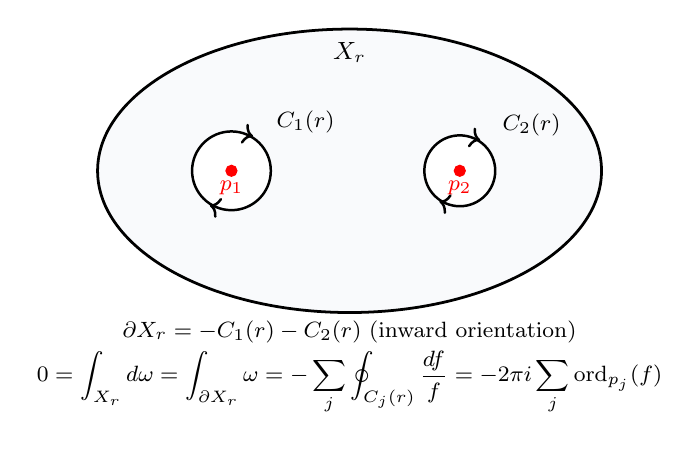
\begin{tikzpicture}[scale=1.0]
  % Surface X_r (filled ellipse, representing the Riemann surface minus disks)
  \fill[softgray!60] (0,0) ellipse (3.2cm and 1.8cm);
  \draw[line width=1pt] (0,0) ellipse (3.2cm and 1.8cm);
  \node[font=\small] at (0, 1.5) {$X_r$};

  % Disk D_1(r) around p_1 (a zero)
  \fill[white] (-1.5, 0) circle (0.5cm);
  \draw[line width=0.9pt,
        decoration={markings,
          mark=at position 0.2 with {\arrow{<}},
          mark=at position 0.7 with {\arrow{<}}
        },
        postaction={decorate}]
    (-1.5, 0) circle (0.5cm);
  \filldraw[red] (-1.5,0) circle (2pt) node[below, font=\footnotesize]{$p_1$};
  \node[font=\footnotesize, above right] at (-1.05, 0.35) {$C_1(r)$};

  % Disk D_2(r) around p_2 (a pole)
  \fill[white] (1.4, 0) circle (0.45cm);
  \draw[line width=0.9pt,
        decoration={markings,
          mark=at position 0.2 with {\arrow{<}},
          mark=at position 0.7 with {\arrow{<}}
        },
        postaction={decorate}]
    (1.4, 0) circle (0.45cm);
  \filldraw[red] (1.4,0) circle (2pt) node[below, font=\footnotesize]{$p_2$};
  \node[font=\footnotesize, above right] at (1.82, 0.32) {$C_2(r)$};

  % Orientation annotation: inward (clockwise) for removed disks
  \node[font=\footnotesize, align=center] at (0,-2.5)
    {$\partial X_r = -C_1(r) - C_2(r)$ (inward orientation)\\[2pt]
     $\displaystyle 0=\int_{X_r}d\omega = \int_{\partial X_r}\omega
       = -\sum_j\oint_{C_j(r)}\frac{df}{f}
       = -2\pi i\sum_j\operatorname{ord}_{p_j}(f)$};
\end{tikzpicture}

\end{center}

% ------ §0.4  Explicit example on CP^1 -----------------
\subsection{An Explicit Example on $\CPone$}
\label{subsec:explicitCP1}

\begin{example}[Winding form of $z-a$]
{\color{blue}Let $f=z-a$ for $a\in\C$.}
In the $z$-chart:
\[
  \frac{d(z-a)}{z-a} = \frac{dz}{z-a},
  \qquad
  \ord_a(f) = \frac{1}{2\pi i}\oint_{\gamma_a}\frac{dz}{z-a} = 1.
\]
Near $\infty$, pass to $w=1/z$:
\[
  \frac{d(z-a)}{z-a}\bigg|_{w=1/z}
  = \frac{-w^{-2}\,dw}{w^{-1}-a}
  = \frac{-w^{-1}\,dw}{1-aw},
  \qquad
  \ord_\infty(f) = -1.
\]
Total: $1+(-1)=0$.\ \checkmark\quad
This verifies Lemma~\ref{lem:degzero} from the winding form directly.
\end{example}

\medskip
\begin{center}
% Tikz-WindingForm.tex
% Winding form on C^× : punctured plane with loop γ, showing (1/2πi)∮dz/z = 1
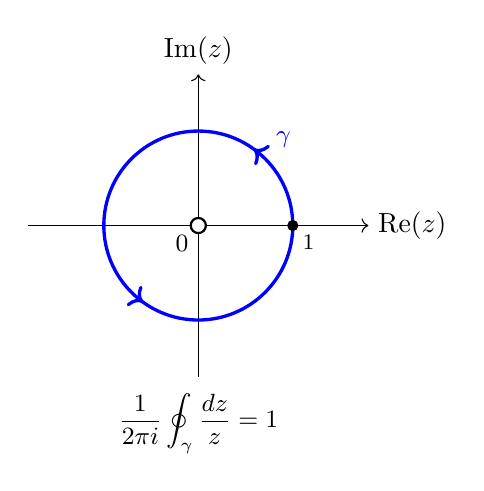
\begin{tikzpicture}[scale=1.2]
  % Axes
  \draw[->] (-1.8,0) -- (1.8,0) node[right] {$\operatorname{Re}(z)$};
  \draw[->] (0,-1.6) -- (0,1.6) node[above] {$\operatorname{Im}(z)$};

  % Puncture at origin
  \filldraw[fill=white, draw=black, line width=0.8pt] (0,0) circle (0.08);
  \node[below left, font=\small] at (0,0) {$0$};

  % Loop γ (unit circle) with counterclockwise arrow
  \draw[line width=1.2pt, blue,
        decoration={markings,
          mark=at position 0.15 with {\arrow[blue]{>}},
          mark=at position 0.65 with {\arrow[blue]{>}}
        },
        postaction={decorate}]
    (0,0) circle (1cm);

  % Label γ
  \node[blue, above right, font=\small] at (0.72, 0.72) {$\gamma$};

  % Annotation: winding integral
  \node[align=center, font=\small] at (0,-2.1)
    {$\displaystyle\frac{1}{2\pi i}\oint_\gamma \frac{dz}{z} = 1$};

  % Small tick at z=1
  \node[below right, font=\footnotesize] at (1,0) {$1$};
  \filldraw (1,0) circle (1.5pt);
\end{tikzpicture}

\end{center}

% ============================================================
%  Section 1: Holomorphic Line Bundles
% ============================================================
\newpage
\section{Holomorphic Line Bundles on $\CPone$}
\label{sec:linebundles}

\medskip\noindent
\emph{Every integer-valued invariant of a line bundle on $\CPone$ is a winding number.}

% ------ §1.1  Transition functions ----------------------
\subsection{Definition via Transition Functions}
\label{subsec:transition}

\defbox[Holomorphic Line Bundle]{%
\begin{definition}
A \textbf{holomorphic line bundle} $\mathcal{L}\to X$ is a rank-$1$ complex vector bundle
with holomorphic transition functions
$g_{ij}:U_i\cap U_j\to\C^\times$
satisfying the cocycle condition $g_{ij}g_{jk}=g_{ik}$ on every triple overlap.
\end{definition}}

\begin{remark}
On $\CPone=U_0\cup U_\infty$, the overlap $U_0\cap U_\infty\cong\C^\times$ has
$\pi_1(\C^\times)\cong\mathbb{Z}$, generated by the unit circle $|z|=1$.
A line bundle is determined (up to isomorphism) by a single transition function
$g_{0\infty}:\C^\times\to\C^\times$, whose homotopy class is its winding number:
\[
  n = \wind{|z|=1}{g_{0\infty}}.
\]
Two transition functions with the same winding number give isomorphic bundles
\textit{(proved in Section~\ref{sec:picard})}.
This is why line bundles on $\CPone$ are classified by $\mathbb{Z}$.
\end{remark}

% ------ §1.2  The bundles O(n) --------------------------
\subsection{The Line Bundles $\mathcal{O}(n)$}
\label{subsec:On}

\defbox[$\mathcal{O}(n)$]{%
\begin{definition}
For $n\in\mathbb{Z}$, the line bundle $\mathcal{O}(n)$ on $\CPone$ has transition function
\[
  g_{0\infty}(z) = z^n.
\]
Special cases:
\begin{itemize}
  \item $\mathcal{O}(0)$: trivial bundle ($g=1$, winding number $0$).
  \item $\mathcal{O}(1)$: hyperplane bundle ($g=z$, winding number $1$).
  \item $\mathcal{O}(-1)$: tautological bundle ($g=z^{-1}$, winding number $-1$).
\end{itemize}
\end{definition}}

\begin{example}[Winding number of $\mathcal{O}(n)$]
From \S\ref{subsec:logderiv}:
\[
  \wind{|z|=1}{(z^n)} = n.
\]
The winding number of the transition function equals the label $n$.\ \checkmark
\end{example}

\begin{observation}
Two transition functions $g=z^n$ and $g'=e^{i\theta}z^n$ give isomorphic bundles because
they differ by a coboundary: set $\phi_0\equiv 1$ on $U_0$ and
$\phi_\infty\equiv e^{i\theta}$ on $U_\infty$.
Then $g'_{0\infty}=\phi_0^{-1}g_{0\infty}\phi_\infty$.
Both $\phi_i$ are holomorphic and nonvanishing on their simply connected charts, so
$\phi_i=e^{h_i}$ for entire functions $h_i$.
The coboundary contributes winding number
\[
  \frac{1}{2\pi i}\oint_{|z|=1}d(h_0-h_\infty) = 0
\]
(integral of an exact form on a closed loop).
Hence only the winding number of $g_{0\infty}$ survives as an invariant.
\end{observation}

% ------ §1.3  Global sections: a winding constraint ----
\subsection{Global Sections: A Winding Constraint}
\label{subsec:sections}

\probox{%
\begin{proposition}
\label{prop:sections}
For $n\geq 0$,
\[
  H^0\!\bigl(\CPone,\,\mathcal{O}(n)\bigr)
  = \operatorname{span}_\C\{1,\,z,\,z^2,\,\ldots,\,z^n\},
  \qquad
  h^0\!\bigl(\mathcal{O}(n)\bigr) = n+1.
\]
For $n<0$, $H^0\!\bigl(\CPone,\,\mathcal{O}(n)\bigr)=0$.
\end{proposition}}

\begin{proof}
A global section is a pair $(s_0,s_\infty)$ of holomorphic functions on $U_0$ and
$U_\infty$ satisfying the gluing condition
\[
  s_0(z) = z^n\cdot s_\infty\!\left(\tfrac{1}{z}\right)
  \quad\text{for all }z\in U_0\cap U_\infty.
\]
\textbf{Step 1.}
{\color{orange}Set $s_0(z)=P(z)$, a holomorphic (hence polynomial) function on $U_0\cong\C$.}
Rearranging the gluing:
\[
  {\color{red}s_\infty(w) = w^n\,P\!\bigl({\textstyle\frac{1}{w}}\bigr).}
\]
\emph{Derivation:} from $s_0(z)=z^n\cdot s_\infty(1/z)$ set $w=1/z$ to get
$s_\infty(w)=w^n s_0(1/w)=w^n P(1/w)$.

\textbf{Step 2.}
$s_\infty$ must be holomorphic at $w=0$ (the point $\infty$).
Write $P(z)=\sum_{k=0}^m a_k z^k$.  Then
\[
  s_\infty(w)=\sum_{k=0}^m a_k\,w^{n-k}.
\]
Holomorphicity at $w=0$ requires $n-k\geq 0$ for every $k\leq m$, i.e., $\deg P\leq n$.

\textbf{Conclusion.}
If $n\geq 0$: $P$ is any polynomial of degree $\leq n$, giving $\operatorname{span}_\C\{1,\ldots,z^n\}$
of dimension $n+1$.
If $n<0$: $\deg P\leq n<0$ forces $P\equiv 0$, so $H^0=0$.
\end{proof}

\begin{infobox}
The gluing $s_0(z)=z^n\cdot s_\infty(1/z)$ is the winding constraint: the section must
\emph{twist $n$ times} as it crosses the equator $|z|=1$.
For $n\geq 0$ there are $n+1$ independent ways to do this; for $n<0$ none.
\end{infobox}

\medskip
\begin{center}
% Tikz-LineBundleGluing.tex
% Two copies of C (charts U_0 and U_∞) glued by w=1/z on the overlap C^×.
% A fiber over the equator |z|=1 shows the twist s_0 = z^n s_∞.
% Inset: winding number computation ∮d(z^n)/z^n = n.
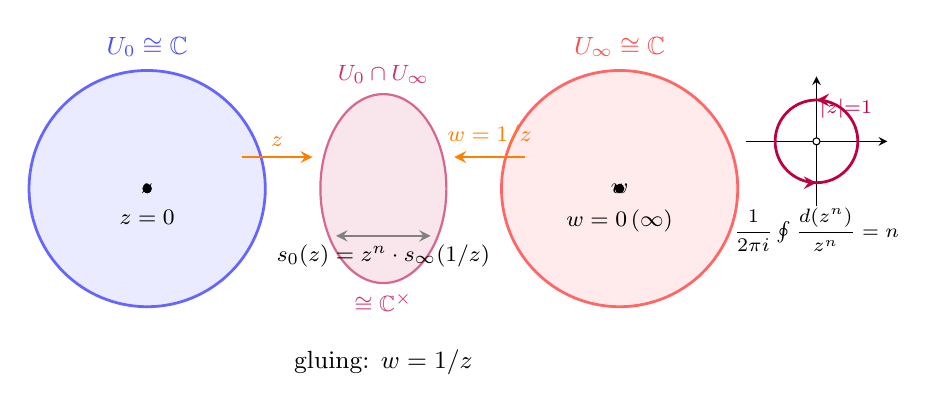
\begin{tikzpicture}[scale=1.0, >=stealth]

  % ── U_0 chart (left disk) ──────────────────────────
  \fill[blue!8] (-3,0) circle (1.5cm);
  \draw[line width=1pt, blue!60] (-3,0) circle (1.5cm);
  \node[font=\small, blue!70] at (-3, 1.8) {$U_0\cong\mathbb{C}$};
  \node[font=\footnotesize] at (-3, 0) {$z$};
  % origin/infinity indication
  \filldraw[black] (-3,0) circle (1.5pt);
  \node[font=\footnotesize, below] at (-3,-0.15) {$z=0$};

  % ── U_∞ chart (right disk) ─────────────────────────
  \fill[red!8] (3,0) circle (1.5cm);
  \draw[line width=1pt, red!60] (3,0) circle (1.5cm);
  \node[font=\small, red!70] at (3, 1.8) {$U_\infty\cong\mathbb{C}$};
  \node[font=\footnotesize] at (3, 0) {$w$};
  \filldraw[black] (3,0) circle (1.5pt);
  \node[font=\footnotesize, below] at (3,-0.15) {$w=0\,(\infty)$};

  % ── Overlap annulus (centre) ───────────────────────
  \fill[purple!10] (0,0) ellipse (0.8cm and 1.2cm);
  \draw[line width=0.8pt, purple!60] (0,0) ellipse (0.8cm and 1.2cm);
  \node[font=\footnotesize, purple!80] at (0, 1.45) {$U_0\cap U_\infty$};
  \node[font=\footnotesize, purple!80] at (0, -1.45) {$\cong\mathbb{C}^\times$};

  % Gluing map w = 1/z
  \draw[->, line width=0.9pt, orange] (-1.8, 0.4) -- (-0.9, 0.4)
    node[midway, above, font=\footnotesize, orange]{$z$};
  \draw[->, line width=0.9pt, orange] (1.8, 0.4) -- (0.9, 0.4)
    node[midway, above, font=\footnotesize, orange]{$w=1/z$};

  % Gluing label
  \node[font=\small] at (0, -2.2) {gluing: $w = 1/z$};

  % ── Fiber twist annotation ─────────────────────────
  \draw[<->, line width=0.8pt, gray] (-0.6, -0.6) -- (0.6, -0.6);
  \node[font=\footnotesize, align=center] at (0, -0.85)
    {$s_0(z) = z^n\cdot s_\infty(1/z)$};

  % ── Winding number inset (top right) ──────────────
  \begin{scope}[shift={(5.5, 0.6)}, scale=0.75]
    \draw[->] (-1.2,0)--(1.2,0);
    \draw[->] (0,-1.1)--(0,1.1);
    \draw[line width=1pt, purple,
          decoration={markings,
            mark=at position 0.25 with {\arrow[purple]{>}},
            mark=at position 0.75 with {\arrow[purple]{>}}
          },
          postaction={decorate}]
      (0,0) circle (0.7cm);
    \filldraw[white, draw=black] (0,0) circle (0.06);
    \node[font=\scriptsize, purple] at (0.5, 0.55) {$|z|{=}1$};
    \node[font=\scriptsize, align=center] at (0,-1.5)
      {$\dfrac{1}{2\pi i}\oint \dfrac{d(z^n)}{z^n}=n$};
  \end{scope}
\end{tikzpicture}

\end{center}

% ============================================================
%  Section 2: Divisors → Line Bundles
% ============================================================
\newpage
\section{From Divisors to Line Bundles}
\label{sec:div2lb}

\medskip\noindent
\emph{A divisor encodes winding data at each point.
This section assembles those data into transition functions and shows that
$H^0(\mathcal{O}(D))=L(D)$.}

% ------ §2.1  O(D) ----------------------------------------
\subsection{The Line Bundle $\mathcal{O}(D)$}
\label{subsec:OD}

\defbox[Line Bundle Associated to a Divisor]{%
\begin{definition}
\label{def:OD}
Let $D=\sum_p n_p[p]\in\Div(\CPone)$.
\begin{enumerate}[(a)]
  \item \textbf{Sheaf of sections.}
    $\mathcal{O}(D)$ assigns to each open $U$ the set
    \[
      \mathcal{O}(D)(U) := \set{f\in\MM(U)^\times:\div(f)\big|_U+D\big|_U\geq 0}\cup\{0\}.
    \]
  \item \textbf{Transition functions (equivalent description).}
    Choose $\{U_i\}$ fine enough that each $U_i$ contains at most one support point of $D$.
    On each $U_i$ pick $\psi_i\in\MM(U_i)^\times$ with $\div(\psi_i)=D|_{U_i}$.
    Set
    \[
      g_{ij}:=\frac{\psi_i}{\psi_j}\quad\text{on }U_i\cap U_j.
    \]
    Then $g_{ij}$ is holomorphic and nonvanishing (since $\div(g_{ij})=D|_{U_i}-D|_{U_j}=0$
    on the overlap) and satisfies the cocycle condition.
\end{enumerate}
\end{definition}}

\begin{remark}[Equivalence of the two descriptions]
A section $s$ of the sheaf over $U_i$ satisfies $\div(s)|_{U_i}+D|_{U_i}\geq 0$,
i.e., $s=\lambda_i\psi_i$ for a holomorphic function $\lambda_i$.
Thus $\lambda_i$ is the fiber coordinate in the $\psi_i$-trivialization, and the
transition $\lambda_i=g_{ij}\lambda_j$ on overlaps recovers the line bundle structure.
The two descriptions define the same object.
\end{remark}

\begin{remark}[Well-definedness]
\label{rem:welldef-OD}
Replacing $\psi_i$ by $f_i\psi_i$ (with $f_i$ holomorphic nonvanishing on $U_i$) gives
$g_{ij}'=f_ig_{ij}f_j^{-1}$, a coboundary with $\phi_k=f_k^{-1}$.
The resulting bundle is isomorphic to the original, so $\mathcal{O}(D)$ is well-defined
as an isomorphism class.
\end{remark}

\begin{observation}[Winding data]
The winding number of $\psi_i$ around a single point $p\in U_i$ is
\[
  \frac{1}{2\pi i}\oint_{\gamma_p}\frac{d\psi_i}{\psi_i}=\ord_p(\psi_i)=n_p.
\]
The transition functions $g_{ij}=\psi_i/\psi_j$ are nonvanishing on overlaps, but the
local trivializations $\psi_i$ carry the winding data of $D$ pointwise.
\end{observation}

\medskip

{\color{blue}\textbf{Concrete case: $D=n[\infty]$.}}
Take $U_0\ni\C$ (which does not contain $\infty$): set $\psi_0=1$.
Take $U_\infty$ with $\infty$ at $w=0$: set $\psi_\infty=w^n$.
On the overlap, with $z=1/w$:
\[
  g_{0\infty}(z) = \frac{\psi_0(z)}{\psi_\infty(1/z)} = \frac{1}{(1/z)^n} = z^n.
\]
Winding number $n$, so $\mathcal{O}(n[\infty])=\mathcal{O}(n)$.\ \checkmark

\thmbox{%
\begin{theorem}
\label{thm:divhom}
The map $D\mapsto\mathcal{O}(D)$ is a group homomorphism
$\Div(\CPone)\to\Pic(\CPone)$.
\end{theorem}}

\begin{proof}
Adding divisors corresponds to multiplying local trivializations:
$\psi_i^{(D+D')}=\psi_i^{(D)}\cdot\psi_i^{(D')}$, and therefore
$g_{ij}^{(D+D')}=g_{ij}^{(D)}\cdot g_{ij}^{(D')}$.
Multiplying transition functions corresponds to tensoring bundles:
$\mathcal{O}(D+D')=\mathcal{O}(D)\otimes\mathcal{O}(D')$.
\end{proof}

% ------ §2.2  H^0 = L(D) --------------------------------
\subsection{Global Sections Recover $L(D)$}
\label{subsec:sectionsLD}

\thmbox{%
\begin{theorem}
\label{thm:H0LD}
$H^0\!\bigl(\CPone,\,\mathcal{O}(D)\bigr) = L(D)$.
\end{theorem}}

\begin{proof}
By Definition~\ref{def:OD}(a), a global section of $\mathcal{O}(D)$ is exactly a
global meromorphic function $f\in\MM(\CPone)$ satisfying $\div(f)+D\geq 0$
(together with the zero function).
This is the definition of $L(D)$.
\end{proof}

\begin{infobox}
The winding form perspective makes $H^0(\mathcal{O}(D))=L(D)$ transparent: both
encode the constraint that the winding number of $f$ at each point $p$ is at
least $-n_p$.
\end{infobox}

% ------ §2.3  Linear equivalence ⟺ isomorphism ----------
\subsection{Linear Equivalence and Isomorphism}
\label{subsec:lineq}

\thmbox{%
\begin{theorem}
\label{thm:lineq}
$D\sim D'\;\iff\;\mathcal{O}(D)\cong\mathcal{O}(D')$.
\end{theorem}}

\begin{proof}
\textbf{($\Rightarrow$)}
Suppose $D-D'=\div(g)$ for some $g\in\MM(\CPone)^\times$.
Take local trivializations $\psi_i$ for $D$.
Define $\psi_i':=\psi_i/g$; then
$\div(\psi_i')=D|_{U_i}-\div(g)|_{U_i}=D'|_{U_i}$.
The transition functions:
\[
  g_{ij}' = \frac{\psi_i'}{\psi_j'}
  = \frac{\psi_i/g}{\psi_j/g} = \frac{\psi_i}{\psi_j} = g_{ij}.
\]
Identical transition functions give isomorphic bundles.

\textbf{($\Leftarrow$)}
If $\mathcal{O}(D)\cong\mathcal{O}(D')$, the isomorphism supplies holomorphic nonvanishing
functions $\phi_i$ on each $U_i$ with $g_{ij}'=\phi_i^{-1}g_{ij}\phi_j$.
Define
\[
  h_i := \frac{\phi_i^{-1}\psi_i}{\psi_i'}\quad\text{on }U_i.
\]
On each overlap $U_i\cap U_j$, using $g_{ij}/g_{ij}'=\phi_i/\phi_j$
(from $g_{ij}'=\phi_i^{-1}g_{ij}\phi_j$):
\[
  \frac{h_i}{h_j}
  = \frac{\phi_j}{\phi_i}\cdot\frac{\psi_i/\psi_i'}{\psi_j/\psi_j'}
  = \frac{\phi_j}{\phi_i}\cdot\frac{g_{ij}}{g_{ij}'}
  = \frac{\phi_j}{\phi_i}\cdot\frac{\phi_i}{\phi_j}
  = 1.
\]
So $h_i$ patches to a global meromorphic $h$.
Its divisor: $\div(h_i)=\div(\phi_i^{-1})+\div(\psi_i)-\div(\psi_i')
=0+D|_{U_i}-D'|_{U_i}=(D-D')|_{U_i}$, giving $\div(h)=D-D'$, hence $D\sim D'$.

\medskip\noindent
\textit{Note:} patching $\psi_i/\psi_i'$ alone fails because
$(\psi_i/\psi_i')/(\psi_j/\psi_j')=g_{ij}/g_{ij}'=\phi_i\phi_j^{-1}\neq 1$ in general;
the coboundary $\phi_i$ from the isomorphism is essential.
\end{proof}

\corbox{%
\begin{corollary}
\label{cor:ellsame}
If $D\sim D'$ then $\ell(D)=\ell(D')$.
\end{corollary}}

\begin{proof}
The isomorphism $\mathcal{O}(D)\cong\mathcal{O}(D')$ induces
$H^0(\mathcal{O}(D))\cong H^0(\mathcal{O}(D'))$, hence $\ell(D)=\ell(D')$ by
Theorem~\ref{thm:H0LD}.
For an explicit vector-space isomorphism: if $\div(g)=D-D'$, then
\[
  \fullfunction{\Phi_g}{L(D)}{L(D')}{f}{gf}
\]
is an isomorphism (see~\cite{RR-CP1} for details).
\end{proof}

% ============================================================
%  Section 3: Picard Group
% ============================================================
\newpage
\section{The Picard Group $\Pic(\CPone)$}
\label{sec:picard}

\medskip\noindent
\emph{The degree of a line bundle is the winding number of its transition function
around the equator.  On $\CPone$ this single integer is the only invariant.}

\subsection{Definition}

\defbox[Picard Group]{%
\begin{definition}
$\Pic(X)$ is the group of isomorphism classes of holomorphic line bundles on $X$,
with group operation $\otimes$ (tensor product) and identity $\mathcal{O}_X$.
The inverse of $[\mathcal{L}]$ is $[\mathcal{L}^{-1}]=[\mathcal{L}^\vee]$.
\end{definition}}

\subsection{The Degree Map as a Winding Number}
\label{subsec:degree}

\defbox[Degree of a Line Bundle]{%
\begin{definition}
\label{def:degree}
The \textbf{degree} of $\mathcal{L}$ with transition function $g_{0\infty}$ is
\[
  \deg\mathcal{L} := \wind{|z|=1}{g_{0\infty}}
  = \frac{1}{2\pi i}\oint_{|z|=1}\frac{dg_{0\infty}}{g_{0\infty}}.
\]
\end{definition}}

\begin{remark}[Well-definedness]
Two representatives of $[\mathcal{L}]$ differ by a coboundary
$g_{0\infty}'=\phi_0^{-1}g_{0\infty}\phi_\infty$, where $\phi_0,\phi_\infty$ are
holomorphic nonvanishing on $U_0\cong\C$ and $U_\infty\cong\C$ respectively.
Both charts are simply connected, so $\phi_i=e^{h_i}$ for entire $h_i$, and the
coboundary contributes
\[
  \frac{1}{2\pi i}\oint_{|z|=1}d(h_\infty-h_0) = 0.
\]
Hence $\deg\mathcal{L}$ is independent of the representative.

\textbf{Important:} the coboundary $\phi_0^{-1}\phi_\infty$ is defined only on the
overlap $U_0\cap U_\infty\cong\C^\times$, not on all of $\CPone$.
Lemma~\ref{lem:degzero} (the degree-zero law) applies to globally defined functions
and cannot be used here; simple connectivity of the charts is the correct tool.
\end{remark}

\begin{remark}[$\deg\mathcal{O}(D)=\deg D$]
\label{rem:degOD}
Assume $D$ has no support on $|z|=1$ (generic).
With $g_{0\infty}=\psi_0/\psi_\infty$ and $d(gg')/(gg')=dg/g+dg'/g'$:
\[
  \frac{1}{2\pi i}\oint_{|z|=1}\frac{dg_{0\infty}}{g_{0\infty}}
  = \underbrace{\frac{1}{2\pi i}\oint_{|z|=1}\frac{d\psi_0}{\psi_0}}_{=\;\sum_{|p|<1}n_p}
  \;-\;
  \underbrace{\frac{1}{2\pi i}\oint_{|z|=1}\frac{d\psi_\infty}{\psi_\infty}}_{
    =\;-\!\sum_{|p|>1\text{ or }p=\infty}\!\!n_p}
  \;=\;\sum_p n_p = \deg D.
\]
The \textbf{first} term is the argument principle (ccw in $z$) counting zeros/poles of
$\psi_0$ inside $|z|<1$.
The \textbf{minus sign} in the second comes from orientation reversal:
$|z|=1$ counterclockwise in $z$ becomes $|w|=1$ \emph{clockwise} in $w=1/z$
(same mechanism as $\partial X_r=-\sum_j C_j(r)$ in \S\ref{subsec:degzero});
the argument principle in the $w$-chart then gives
$-\sum_{|p|>1\text{ or }p=\infty}n_p$.
\end{remark}

\probox{%
\begin{proposition}
\label{prop:deghom}
$\deg:\Pic(\CPone)\to\mathbb{Z}$ is a group homomorphism.
\end{proposition}}

\begin{proof}
The tensor product $\mathcal{L}\otimes\mathcal{L}'$ has transition function $gg'$, and
\[
  \frac{d(gg')}{gg'} = \frac{dg}{g}+\frac{dg'}{g'},
\]
so $\deg(\mathcal{L}\otimes\mathcal{L}')=\deg\mathcal{L}+\deg\mathcal{L}'$.
\end{proof}

\subsection{$\Pic(\CPone)\cong\mathbb{Z}$}
\label{subsec:Piciso}

\thmbox{%
\begin{theorem}
\label{thm:Pic}
\[
  \fullfunction{\Phi}{\Pic(\CPone)}{\mathbb{Z}}{[\mathcal{L}]}{\deg\mathcal{L}}
\]
is a group isomorphism.
\end{theorem}}

\begin{proof}
\textbf{Key lemma} (proved in~\cite{RR-CP1}):
\emph{every divisor $D$ on $\CPone$ satisfies $D\sim(\deg D)[\infty]$.}
The proof uses $\div(z-a)=[a]-[\infty]$ to move each finite point to $[\infty]$.
This single lemma yields both surjectivity and injectivity without circularity.

\medskip
\textbf{Surjectivity:}
$z^n$ achieves every integer winding number, so $\mathcal{O}(n)$ is a line bundle of
degree $n$ for every $n\in\mathbb{Z}$.

\medskip
\textbf{Injectivity:}
Suppose $\deg[\mathcal{L}]=n$.
Any line bundle $\mathcal{L}$ of degree $n$ has a meromorphic section $s$
(for $\mathcal{O}(n)$ this is explicit; for general $\mathcal{L}$ this follows from the
construction in Definition~\ref{def:OD}).
The divisor $D':=\div(s)+n[\infty]$ satisfies $\mathcal{O}(D')\cong\mathcal{L}$.
By the key lemma, $D'\sim n[\infty]$, so by Theorem~\ref{thm:lineq},
$\mathcal{L}\cong\mathcal{O}(D')\cong\mathcal{O}(n[\infty])=\mathcal{O}(n)$.
Hence every degree-$n$ line bundle is isomorphic to $\mathcal{O}(n)$, so degree is a
complete invariant.

\medskip
\textbf{Why no circular dependency:}
The surjectivity of $\Div\to\Pic$ (every line bundle comes from a divisor)
also follows from the key lemma: $\mathcal{O}(n)=\mathcal{O}(n[\infty])$ comes from
$n[\infty]$.
This is independent of the injectivity argument; the key lemma is the sole input.
\end{proof}

\begin{greenboxenv}
\textbf{Why $\CPone$ is the simplest case.}
On a genus-$g$ curve, the degree map $\deg:\Pic(X)\to\mathbb{Z}$ exists, but its
kernel $\Pic^0(X)$ (degree-$0$ line bundles) is a $g$-dimensional complex torus
(the Jacobian).
For $\CPone$ ($g=0$), Theorem~\ref{thm:Pic} says $\Pic^0(\CPone)=0$: every degree-$0$
bundle is trivial because $D\sim 0$ whenever $\deg D=0$.
This is the sense in which $\CPone$ is the simplest compact Riemann surface.
\end{greenboxenv}

\medskip
\begin{center}
% Tikz-PicardGroup.tex
% Integer number line labelling O(n) at each node.
% Winding number n = (1/2πi)∮ dg/g written below.
% Arrow shows O(n) ⊗ O(m) = O(n+m).
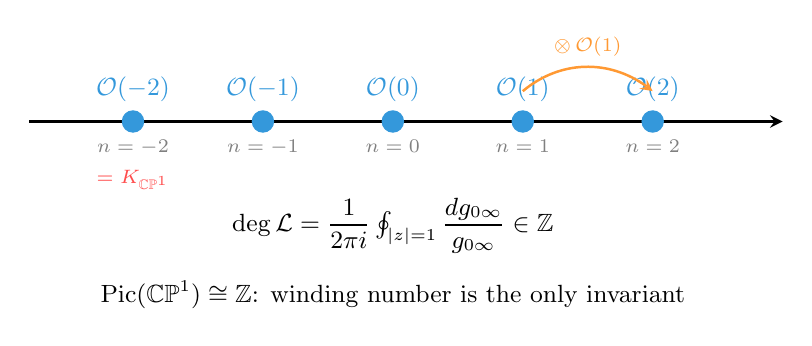
\begin{tikzpicture}[scale=1.1, >=stealth]

  % Number line
  \draw[line width=1pt, ->] (-4.2,0) -- (4.5,0);

  % Nodes n = -2, -1, 0, 1, 2
  \foreach \n/\lbl in {-2/{-2}, -1/{-1}, 0/{0}, 1/{1}, 2/{2}}{
    \filldraw[defcolor] (\n*1.5, 0) circle (3.5pt);
    % O(n) label above
    \node[above, font=\small, defcolor] at (\n*1.5, 0.12)
      {$\mathcal{O}(\lbl)$};
    % winding number label below
    \node[below, font=\scriptsize, gray] at (\n*1.5, -0.1)
      {$n=\lbl$};
  }

  % Special label for K = O(-2)
  \node[below, font=\scriptsize, red!70] at (-3, -0.45)
    {$=K_{\mathbb{CP}^1}$};

  % Tensor product arrow: O(1) ⊗ O(1) = O(2)
  \draw[->, line width=0.9pt, orange!80, bend left=40]
    (1.5, 0.35) to node[above, font=\scriptsize, orange!80]
    {$\otimes\,\mathcal{O}(1)$} (3.0, 0.35);

  % Winding number formula at bottom
  \node[font=\small, align=center] at (0, -1.2)
    {$\deg\mathcal{L}
       = \dfrac{1}{2\pi i}\oint_{|z|=1}\dfrac{dg_{0\infty}}{g_{0\infty}}
       \in \mathbb{Z}$};

  % Isomorphism label
  \node[font=\small] at (0, -2.0)
    {$\Pic(\mathbb{CP}^1)\cong\mathbb{Z}$: winding number is the only invariant};

\end{tikzpicture}

\end{center}

\subsection{The Short Exact Sequence}
\label{subsec:ses}

\begin{remark}
By Liouville's theorem, every holomorphic function on the compact surface $\CPone$
is constant, so $\OO(\CPone)^\times=\C^\times$.
There are no nontrivial globally holomorphic gauge transformations on $\CPone$.
\end{remark}

\probox{%
\begin{proposition}
There is a short exact sequence
\[
  0 \;\to\; \C^\times
    \;\to\; \MM(\CPone)^\times
    \;\xrightarrow{\;\div\;}\; \Div(\CPone)
    \;\to\; \Pic(\CPone)
    \;\to\; 0.
\]
\end{proposition}}

\begin{proof}[Proof (sketch)]
\emph{Exactness at $\MM^\times$:}
A function with all winding numbers $\ord_p(f)=0$ has $\div(f)=0$, hence is holomorphic
and nonvanishing on compact $\CPone$, hence constant.

\emph{Exactness at $\Div$:}
By definition, $\operatorname{image}(\div)=\Prin(\CPone)=\ker(\Div\to\Pic)$.

\emph{Exactness at $\Pic$:}
Every $\mathcal{O}(n)=\mathcal{O}(n[\infty])$ comes from the divisor $n[\infty]$,
so $\Div\to\Pic$ is surjective.
\end{proof}

\begin{warningbox}
Exactness at $\Pic(\CPone)$ — every line bundle arises from a divisor — requires
$H^1(\CPone,\MM^\times)=0$.
This follows from Theorem~\ref{thm:Pic} (every bundle is $\mathcal{O}(n[\infty])$),
not from any formal property of the exact sequence alone.
\end{warningbox}

% ============================================================
%  Section 4: Canonical Bundle and Serre Duality
% ============================================================
\newpage
\section{The Canonical Bundle and Serre Duality}
\label{sec:canonical}

\medskip\noindent
\emph{The canonical bundle is determined by how $1$-forms transform on the overlap
— another winding number calculation.}

\subsection{The Canonical Bundle $K_{\CPone}$}
\label{subsec:canonical}

\defbox[Canonical Bundle]{%
\begin{definition}
The \textbf{canonical bundle} $K_X=\Omega^1_X$ is the cotangent line bundle;
its sections over $U$ are holomorphic $1$-forms on $U$.
\end{definition}}

\begin{remark}[Transition function via the winding form]
On $U_0\cap U_\infty$, a $1$-form $f(z)\,dz$ in the $z$-trivialization transforms
via $w=1/z$:
\[
  f(z)\,dz
  = f\!\left(\tfrac{1}{w}\right)\cdot d\!\left(\tfrac{1}{w}\right)
  = f\!\left(\tfrac{1}{w}\right)\cdot\left(-\frac{1}{w^2}\right)dw
  = -\frac{f(1/w)}{w^2}\,dw.
\]
The section in the $w$-trivialization is $s_\infty(w)=-f(1/w)/w^2$.
The gluing $s_0(z)=g^K_{0\infty}(z)\cdot s_\infty(1/z)$ gives
$f(z)=g^K_{0\infty}(z)\cdot(-z^2 f(z))$, hence
\[
  g^K_{0\infty}(z) = -z^{-2}.
\]
The winding number: since $d(-z^{-2})=2z^{-3}\,dz$,
\[
  \deg K
  = \frac{1}{2\pi i}\oint_{|z|=1}\frac{d(-z^{-2})}{-z^{-2}}
  = \frac{1}{2\pi i}\oint_{|z|=1}\frac{2z^{-3}\,dz}{-z^{-2}}
  = \frac{1}{2\pi i}\oint_{|z|=1}\frac{-2\,dz}{z}
  = -2.
\]
Therefore $K_{\CPone}=\mathcal{O}(-2)$.
\end{remark}

\begin{observation}[Consistency check via $dz/z$]
In the $z$-chart, $dz/z$ has a simple pole at $0$.
In the $w$-chart ($w=1/z$): $\dfrac{dz}{z}=\dfrac{-w^{-2}\,dw}{w^{-1}}=-\dfrac{dw}{w}$,
a simple pole at $w=0$ (i.e., at $\infty$).
So
\[
  \div\!\left(\frac{dz}{z}\right) = -[0]-[\infty],
  \qquad
  \deg = -2 = \deg K.\ \checkmark
\]
All meromorphic $1$-forms on $\CPone$ have divisor of degree $-2$;
none are holomorphic everywhere, consistent with
$h^0(K)=\ell(K)=\max(0,-2+1)=0$.
\end{observation}

\begin{remark}
$\deg K=-2$ is consistent with $g=0$ and the \textbf{genus formula}
$\deg K=2g-2$ (a consequence of Gauss--Bonnet applied to the curvature of $K_X$).
Riemann--Hurwitz, which governs ramification of covering maps, is the wrong reference here.
\end{remark}

\subsection{Serre Duality}
\label{subsec:serre}

\thmbox{%
\begin{theorem}[Serre Duality — statement only]
\label{thm:serre}
For a holomorphic line bundle $\mathcal{L}$ on a compact Riemann surface $X$,
\[
  H^1(X,\mathcal{L})\cong H^0\!\bigl(X,\,K_X\otimes\mathcal{L}^{-1}\bigr)^\vee
\]
as $\C$-vector spaces, where $(-)^\vee=\operatorname{Hom}_\C(-,\C)$.
\end{theorem}}

\begin{warningbox}
The proof of Serre duality requires fine sheaves, the $\bar\partial$-operator, and
elliptic regularity.  It is deferred.
\end{warningbox}

\begin{remark}[Consequence for $\CPone$]
\label{rem:serre-CP1}
With $\mathcal{L}=\mathcal{O}(n)$ and $K_{\CPone}=\mathcal{O}(-2)$:
\[
  H^1\!\bigl(\CPone,\,\mathcal{O}(n)\bigr)
  \cong H^0\!\bigl(\CPone,\,\mathcal{O}(-n-2)\bigr)^\vee.
\]
Taking dimensions (the dual has the same dimension):
\[
  h^1\!\bigl(\mathcal{O}(n)\bigr) = h^0\!\bigl(\mathcal{O}(-n-2)\bigr) = \max(0,\,-n-1).
\]
\end{remark}

% ============================================================
%  Section 5: Riemann–Roch
% ============================================================
\newpage
\section{Riemann--Roch Theorem on $\CPone$}
\label{sec:RR}

\subsection{Statement}

\begin{infobox}
On a compact Riemann surface $X$ of genus $g$:
\[
  \ell(D) - \ell(K-D) = \deg D + 1 - g.
\]
For $X=\CPone$ ($g=0$):
\[
  \ell(D)-\ell(K-D)=\deg D + 1.
\]
Viewed as a winding-number balance:
\[
  \underbrace{\ell(D)}_{\text{sections: }\ord_p\geq -n_p}
  -
  \underbrace{\ell(K-D)}_{h^1\text{ via Serre duality}}
  =
  \underbrace{\deg D}_{\text{total winding}}
  +\;1.
\]
\end{infobox}

\thmbox{%
\begin{theorem}[Riemann--Roch on $\CPone$]
\label{thm:RR}
For every $D\in\Div(\CPone)$,
\[
  \ell(D) - \ell(K-D) = \deg D + 1.
\]
\end{theorem}}

\subsection{Proof via Winding Numbers}

\begin{proof}
\textbf{Step 1: Reduce to $D=n[\infty]$.}
Every finite point satisfies $[a]\sim[\infty]$ via $\div(z-a)=[a]-[\infty]$
(the winding form $d(z-a)/(z-a)$ has winding $+1$ at $a$ and $-1$ at $\infty$).
Applying repeatedly, every $D$ of degree $n$ satisfies $D\sim n[\infty]$.
By Corollary~\ref{cor:ellsame}: $\ell(D)=\ell(n[\infty])$ and
$\ell(K-D)=\ell(K-n[\infty])$.

\textbf{Step 2: Compute $\ell(n[\infty])$.}
By Proposition~\ref{prop:sections},
$\ell(n[\infty])=\max(0,n+1)$.

\textbf{Step 3: Identify the canonical divisor.}
$K_{\CPone}=\mathcal{O}(-2)$ has degree $-2$ (\S\ref{subsec:canonical}).
By Theorem~\ref{thm:Pic} ($\Pic^0(\CPone)=0$), the unique degree-$(-2)$ bundle is
$\mathcal{O}(-2)=\mathcal{O}(-2[\infty])$, so take $K=-2[\infty]$.
Then $K-D\sim(-n-2)[\infty]$, and
$\ell(K-D)=\max(0,-n-1)$.

\textbf{Step 4: Verify case by case.}
\begin{enumerate}[(i)]
  \item {\color{blue}$n\geq 0$:}
    $\ell(D)=n+1$,\; $\ell(K-D)=0$ (since $-n-1<0$).
    $(n+1)-0=n+1$.\ \checkmark
  \item {\color{blue}$n=-1$:}
    $\ell(D)=\max(0,0)=0$,\;
    $\ell(K-D)=\ell(-[\infty])=\max(0,0)=0$.
    $0-0=0=-1+1$.\ \checkmark
  \item {\color{blue}$n\leq -2$:}
    $\ell(D)=0$,\;
    $\ell(K-D)=\max(0,-n-1)=-n-1>0$.
    $0-(-n-1)=n+1$.\ \checkmark
\end{enumerate}
\end{proof}

\begin{infobox}
Riemann--Roch on $\CPone$ is a bookkeeping identity for winding numbers: the number
of independent sections of $\mathcal{O}(n)$ minus the number of independent correction
sections equals the total winding $n$ plus one.
\end{infobox}

\subsection{Cohomological Reformulation}
\label{subsec:cohRR}

\probox{%
\begin{proposition}
Riemann--Roch on $\CPone$ is equivalent to
\[
  h^0\!\bigl(\mathcal{O}(D)\bigr) - h^1\!\bigl(\mathcal{O}(D)\bigr) = \deg D + 1.
\]
\end{proposition}}

\begin{proof}
$h^0(\mathcal{O}(D))=\ell(D)$ by Theorem~\ref{thm:H0LD}.
By Serre duality (Theorem~\ref{thm:serre}) the vector-space isomorphism
$H^1(\CPone,\mathcal{O}(n))\cong H^0(\CPone,\mathcal{O}(-n-2))^\vee$
gives the dimension equality
$h^1(\mathcal{O}(n))=h^0(\mathcal{O}(-n-2))=\ell(K-D)$
(Remark~\ref{rem:serre-CP1}).
Substituting into Theorem~\ref{thm:RR} yields the result.
\end{proof}

\begin{observation}
Three distinct regimes:
\begin{itemize}
  \item {\color{blue}$n\geq 0$:}
    $\ell(D)=n+1>0$ and $h^1=0$.
    Riemann--Roch is the clean count $h^0=\deg D+1$.
  \item {\color{blue}$n=-1$:}
    $\ell(D)=0$ and $h^1=0$.
    Both sides are $0$; Riemann--Roch holds trivially.
  \item {\color{blue}$n\leq -2$:}
    $\ell(D)=0$ and $h^1=-n-1>0$.
    Serre duality ``reflects'' the count: $0-(-n-1)=n+1$.
\end{itemize}
\textbf{Causal order:} $\ell(D)=0$ already at $n=-1$, independently of $h^1$.
The $h^1$ obstruction activates only at $n\leq -2$; it does not \emph{cause}
$\ell(D)$ to vanish, but accounts for the deficit $\deg D+1<0$ once $\ell(D)$
is already zero.
\end{observation}

\medskip
\begin{center}
% Tikz-RiemannRoch-Balance.tex
% Graph of ℓ(D) and ℓ(K-D) vs n = deg D.
% ℓ(D)   = max(0, n+1)  : zero for n < 0, ramp for n ≥ 0
% ℓ(K-D) = max(0,-n-1)  : ramp for n ≤ -2, zero for n ≥ -1
% Vertical gap = n+1 for all n.
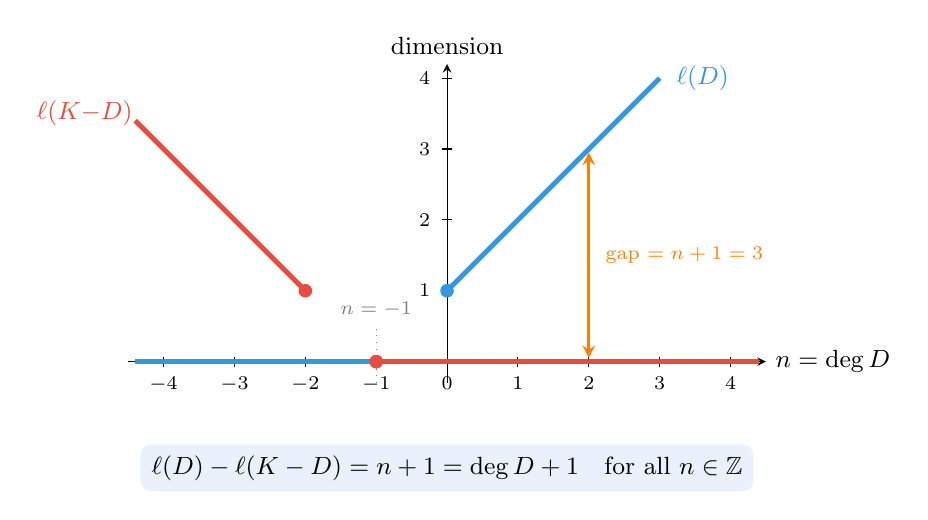
\begin{tikzpicture}[scale=0.9, >=stealth]

  % Axes
  \draw[->] (-4.5,0) -- (4.5,0) node[right, font=\small] {$n=\deg D$};
  \draw[->] (0,-0.3) -- (0,4.2) node[above, font=\small] {dimension};

  % Tick marks on x-axis
  \foreach \x/\lbl in {-4/{-4},-3/{-3},-2/{-2},-1/{-1},0/{0},1/{1},2/{2},3/{3},4/{4}}{
    \draw (\x, 0.07) -- (\x, -0.07);
    \node[below, font=\scriptsize] at (\x, -0.08) {$\lbl$};
  }

  % Tick marks on y-axis
  \foreach \y in {1,2,3,4}{
    \draw (0.07,\y) -- (-0.07,\y);
    \node[left, font=\scriptsize] at (-0.1,\y) {$\y$};
  }

  % ── ℓ(D) = max(0, n+1) : blue ────────────────────
  % flat 0 for n ≤ -1
  \draw[line width=1.8pt, defcolor] (-4.4, 0) -- (-1, 0);
  % ramp for n ≥ 0: (0,1),(1,2),(2,3),(3,4)
  \draw[line width=1.8pt, defcolor] (0,1) -- (3,4);
  % dot at transition
  \filldraw[defcolor] (0,1) circle (2.5pt);
  \filldraw[defcolor] (-1,0) circle (2.5pt);
  \node[defcolor, right, font=\small] at (3.1, 4.0) {$\ell(D)$};

  % ── ℓ(K-D) = max(0,-n-1) : red ───────────────────
  % flat 0 for n ≥ -1
  \draw[line width=1.8pt, thmcolor] (-1, 0) -- (4.4, 0);
  % ramp for n ≤ -2: (-2,1),(-3,2),(-4,3)
  \draw[line width=1.8pt, thmcolor] (-2,1) -- (-4.4, 3.4);
  \filldraw[thmcolor] (-2,1) circle (2.5pt);
  \filldraw[thmcolor] (-1,0) circle (2.5pt);
  \node[thmcolor, left, font=\small] at (-4.3, 3.5) {$\ell(K{-}D)$};

  % ── Vertical gap annotation at n=2 ────────────────
  \draw[<->, orange, line width=1pt] (2, 0.05) -- (2, 2.95);
  \node[orange, right, font=\scriptsize] at (2.1, 1.5)
    {gap $= n+1 = 3$};

  % n = -1: both zero
  \draw[dotted, gray] (-1,-0.3) -- (-1, 0.5);
  \node[font=\scriptsize, gray, above] at (-1, 0.5) {$n=-1$};

  % Formula box
  \node[fill=noteblue, rounded corners, font=\small, inner sep=4pt,
        align=center] at (0,-1.5)
    {$\ell(D) - \ell(K-D) = n+1 = \deg D + 1$\quad for all $n\in\mathbb{Z}$};

\end{tikzpicture}

\end{center}

% ============================================================
%  Section 6: Examples and Applications
% ============================================================
\newpage
\section{Examples and Applications}
\label{sec:examples}

\subsection{Table of $\mathcal{O}(n)$ Sections}

\begin{center}
\renewcommand{\arraystretch}{1.3}
\begin{tabular}{c|c|c|l}
  \toprule
  $n$ & Bundle & $\ell(n[\infty])$ & Basis of $H^0(\mathcal{O}(n))$ \\
  \midrule
  $n\leq -1$ & $\mathcal{O}(n)$          & $0$   & $\emptyset$ \\
  $-2$       & $K_{\CPone}=\mathcal{O}(-2)$ & $0$  & $\emptyset$ \\
  $-1$       & $\mathcal{O}(-1)$          & $0$   & $\emptyset$ \\
  $0$        & $\mathcal{O}_{\CPone}$     & $1$   & $\{1\}$ \\
  $1$        & $\mathcal{O}(1)$           & $2$   & $\{1,\,z\}$ \\
  $2$        & $\mathcal{O}(2)$           & $3$   & $\{1,\,z,\,z^2\}$ \\
  $n\geq 0$  & $\mathcal{O}(n)$           & $n+1$ & $\{1,\,z,\,\ldots,\,z^n\}$ \\
  \bottomrule
\end{tabular}
\end{center}

\subsection{Verifying Riemann--Roch on Specific Divisors}

The following three examples revisit computations from~\cite{RR-CP1}
and restate them in terms of line bundles.
Throughout, the affine point $z_0\in\C$ corresponds to $[1:z_0]\in\CPone$.

\begin{example}[{$D=[0]$}]
$\deg D=1$, so $\mathcal{O}([0])\cong\mathcal{O}(1)$.
By Proposition~\ref{prop:sections}: $\ell=1+1=2$, basis $\{1,z\}$.
Riemann--Roch: $2-0=1+1$.\ \checkmark
\end{example}

\begin{example}[{$D=[0]+[1]$}]
$\deg D=2$, so $\mathcal{O}([0]+[1])\cong\mathcal{O}(2)$.
$\ell=2+1=3$, basis $\{1,z,z^2\}$.
Riemann--Roch: $3-0=2+1$.\ \checkmark
\end{example}

\begin{example}[{$D=[\infty]-[1]$}]
$\deg D=0$, so $\mathcal{O}([\infty]-[1])\cong\mathcal{O}(0)=\mathcal{O}$.
$\ell=\max(0,1)=1$, basis $\{1\}$ (constants).
Cross-check from~\cite{RR-CP1}: $L([\infty]-[1])=\operatorname{span}_\C\{z-1\}$,
dimension $1$.\ \checkmark
Riemann--Roch: $1-0=0+1$.\ \checkmark
\end{example}

\subsection{Morphisms to Projective Space}

\probox{%
\begin{proposition}
If $\deg D\geq 1$ on $\CPone$, a basis $\{f_0,\ldots,f_m\}$ of $L(D)$
($m=\ell(D)-1$) defines a morphism
\[
  \phi_D:\CPone\to\mathbb{P}^m,\qquad
  p\mapsto [f_0(p):\cdots:f_m(p)].
\]
The base locus is empty since the constant function $1\in L(D)$ never vanishes.
\end{proposition}}

Convention: the affine point $z\in\C$ corresponds to the homogeneous point
$[1:z]\in\CPone$.

\begin{example}[{$D=[\infty]$}, identity map]
Basis $\{1,z\}$, target $\mathbb{P}^1$.
\[
  \phi:\,[1:z_0]\mapsto [1\,{:}\,z_0].
\]
This is the identity $\CPone\xrightarrow{\sim}\CPone$.
\end{example}

\begin{example}[{$D=2[\infty]$}, Veronese embedding]
Basis $\{1,z,z^2\}$, target $\mathbb{P}^2$.
\[
  \phi:\,[1:z]\mapsto [1:z:z^2].
\]
The image is the conic $\{[X:Y:Z]\in\mathbb{P}^2:XZ=Y^2\}$.
\end{example}

% ── Bibliography ──────────────────────────────────────────
\begin{thebibliography}{9}
\bibitem{RR-CP1}
Ji, Yonghyeon.
\textit{Riemann--Roch Theorem on $\mathbb{CP}^1$}.
Lecture notes, 2025.
\end{thebibliography}

\end{document}
